 %%% Lezione 13


\lecture[Dimostrazione del teorema sull'esistenza della successione spettrale associata ad un complesso filtrato. Applicazione delle successioni spettrali.]{2023-04-17}

Dato un complesso di catene \emph{filtrato} e \emph{graduato} $(A,d,f)$,
questo determina in maniera naturale una successione spettrale:
una volta capito il ``modo giusto'' per mettere d'accordo il grado
(co)omologico e il grado della filtrazione, il seguente \textbf{Teorema}
fornisce un macchinario per costruire successioni spettrali.

\begin{thm}\label{SS-machine}
	Un complesso di catene graduato e filtrato $(A,d,F)$ determina una successione spettrale
	$\Set{(E_{\bullet,\bullet}^{r},d^{r}) | r = 1, 2, \dots}$,
	con $d^{r}$ di bigrado $(-r, r-1)$, tale che
	\begin{equation*}
		E_{s,t}^{1} = H_{s+t}(F_{s}A/F_{s-1}A)
	\end{equation*}
	e il differenziale $d^{1}$ è
	l'\textbf{omomorfismo di connessione} della tripla $(F_{s}A,F_{s-1}A,F_{s-2}A)$.
	Se la filtrazione $F$ è convergente e limitata sia dal basso, sia dall'alto,
	allora la successione spettrale stabilizza. Inoltre, il limite è
	$$E^{\infty}_{p,q} \simeq \frac{F_{p}H_{p+q}(A,d)}{F_{p-1}H_{p+q}(A,d)}\,.$$
\end{thm}

\begin{oss}
	Ricordiamo che cosa si intende con \textbf{omomorfismo di connessione}
	della tripla $(F_{s}A,F_{s-1}A,F_{s-2}A)$: 
	dato che i moduli graduati $F_{s}A$ sono dotati di un differenziale,
	possono essere considerati come complessi di catene,
	quindi la successione esatta corta
	\begin{equation*}
		\begin{tikzcd}
			\cat{0} \ar[r]
			& \frac{F_{s-1}A}{F_{s-2}A} \ar[r]
			& \frac{F_{s}A}{F_{s-2}A} \ar[r]
			& \frac{F_{s}A}{F_{s-1}A} \ar[r]
			& \cat{0}
		\end{tikzcd}
	\end{equation*}
	induce la successione esatta lunga in omologia
	\begin{equation*}
		\begin{tikzcd}[column sep=small]
			\dots \ar[r]
			& H_{i}\left( \frac{F_{s}A}{F_{s-2}A} \right) \ar[r]
			& H_{i}\left( \frac{F_{s}A}{F_{s-1}A} \right) \ar[r, "\de"]
			& H_{i-1}\left( \frac{F_{s-1}A}{F_{s-2}A} \right) \ar[r]
			& H_{i-1}\left( \frac{F_{s}A}{F_{s-2}A} \right) \ar[r]
			& \dots
		\end{tikzcd}
	\end{equation*}
	per il \textbf{Lemma del Serpente}. 
	La mappa $\de :  H_{i}\left( F_{s}A/F_{s-1}A \right) \to 
	H_{i-1}\left( F_{s-1}A/F_{s-2}A \right)$ nella successione sopra
	è detto \textbf{omomorfismo di connessione}.
\end{oss}	

\begin{oss}
	L'enunciato del \hyperref[SS-machine]{Teorema~\ref{SS-machine}}
	può essere adattato a \emph{complessi di cocatene},
	i quali determinano una successione spettrale in \textbf{coomologia}.
\end{oss}
	
\begin{proof}[Dimostrazione del Teorema~\ref{SS-machine}]
	Partendo dal differenziale $d$ del complesso $A$, che ha grado $-1$,
	l'idea della costruzione consiste nel definire opportuni sottomoduli
	$Z^{r}_{s,t}$ di $A$ in modo tale che, restringendo il differenziale $d$
	a $Z^{r}_{s,t}$, questo sia obbligato ad avere immagine in $Z^{r}_{s-r,t+r-1}$.
	Dopodiché si verifica che queste definizioni producono una successione
	spettrale in cui valgono gli isomorfismi enunciati.
	
	Ricordiamo che su $A$ abbiamo una filtrazione crescente
	\begin{equation*}
		\dots \subset F_{s-1}A \subset F_{s}A \subset F_{s+1}A \subset \dots
	\end{equation*}
		Poniamo
		\begin{equation*}
			Z_{s,t}^{r} = \Set{c \in F_{s}A_{s+t} | dc \in F_{s-r}A_{s+t-1}}
			= F_{s}A_{s+t} \cap d^{-1}\left(F_{s-r}A_{s+t-1}\right) \,,
		\end{equation*}
		il modulo degli elementi di $F_{s}A_{s+t}$ che hanno bordo
		in $F_{s-r}A_{s+t-1}$ (si noti che è l'apice in alto a
		farci capire di quanto shifta il grado della filtrazione).
		Invece, gli elementi di $F_{s}A_{s+t}$
		che non hanno bordo saranno denotati con
		\begin{equation*}
			Z_{s,t}^{\infty} := \Set{c \in F_{s}A_{s+t} | dc = 0} = \ker d \cap F_{s}A_{s+t}\,.
		\end{equation*}
		Per definire l'elemento $E^{r}_{s,t}$ della successione spettrale,
		in $Z_{s,t}^{r}$ eliminiamo sia gli elementi che sono bordi di
		qualche modulo $(r-1)$-esimo, sia quegli elementi di $Z^{r-1}$ che 
		vengono mandati in $F_{s-r}A_{s+t-1}$ dal differenziale: più precisamente,
		notiamo che 
		\begin{equation*}
			c \in Z^{r-1}_{s+r-1,t-r+2} \implies dc \in F_{s}A_{s+t}
		\end{equation*}
		e in particolare $dc \in Z_{s,t}^{r}$ dato che $d^{2}=0$,
		e anche
		\begin{equation*}
			c \in Z^{r-1}_{s-1,t+1} \implies
			c \in F_{s-1}A_{s+t} \subset F_{s}A_{s+t}
			\text{ e inoltre } dc \in F_{s-r}A_{s+t-1}\,.
		\end{equation*}
		Si definisce quindi
		\begin{equation*}
			E^{r}_{s,t} := \left. Z_{s,t}^{r} \middle/ 
			(Z_{s-1, t+1}^{r-1} + dZ^{r-1}_{s+r-1, t-r+2}) \right.
		\end{equation*}
		e analogamente il termine ``\emph{limite}'''
			\begin{equation*}
				E^{\infty}_{s,t} := \left. Z^{\infty}_{s,t} \middle/ 
				\big( Z_{s-1,t+1}^{\infty} + (dA_{s+t+1} \cap F_{s}A_{s+t}) \big) \right. \,.
			\end{equation*}
		In questo modo il differenziale
			$d: Z^{r}_{s,t} \to Z_{s-r, t+r-1}^{r}$
		ha bigrado $(-r,r-1)$ e per costruzione induce
		\begin{equation*}
		 	d^{r} : E^{r}_{s,t} \longrightarrow E^{r}_{s-r,t+r-1} \,.
		 \end{equation*} 
		Calcoliamo i primi passaggi per capire cosa succede: 
		per ogni $r \ge 0$, dato che $F$ è una filtrazione crescente, si ha
		\begin{equation*}
			Z^{-r}_{s,t} = \Set{ c \in F_{s}A_{s+t} | dc \in F_{s+r}A_{s+t-1} } = F_{s}A_{s+t}\,,
		\end{equation*}
		dunque la $0$-esima pagina della successione spettrale è data da
		\begin{equation*}
			E_{s,t}^{0} = F_{s}A_{s+t}/F_{s-1}A_{s+t}\,, \qquad
			d^{0}: F_{s}A_{s+t}/F_{s-1}A_{s+t} \longrightarrow F_{s}A_{s+t-1}/F_{s-1}A_{s+t-1}\,,
		\end{equation*}
		dove il differenziale è indotto da $d$. La prima pagina è stata definita come
		\begin{equation*}
			E_{s,t}^{1} = Z_{s,t}^{1}/(Z_{s-1, t+1}^{0} + dZ_{s,t+1}^{0})
			= Z^{1}_{s,t}/( F_{s-1}A_{s+t} + dF_{s}A_{s+t+1} ) \,;
		\end{equation*}
		notiamo che $Z^{1}_{s,t}/Z^{0}_{s-1,t+1}$ sono i \emph{cicli} 
		di $F_{s}A_{s+t}/F_{s-1}A_{s+t}$,
		mentre $(Z^{0}_{s-1,t+1} + dZ_{s,t}^{0})/Z^{0}_{s-1,t+1}$ sono 
		i \emph{bordi} di $F_{s}A_{s+t}/F_{s-1}A_{s+t}$.
		Ne segue che l'inclusione $Z_{s,t}^{1} \to F_{s}A_{s+t}$ induce un isomorfismo
		\begin{equation*}
			E^{1}_{s,t} \simeq H_{s+t}\left( F_{s}A/F_{s-1}A \right)\,,
		\end{equation*}
		e il differenziale indotto da $d$ è l'omomorfismo di connessione della tripla
		$(F_{s}A, F_{s-1}A, F_{s-2}A)$: infatti, le due righe centrali del diagramma
		\begin{equation*}
			\begin{tikzcd}
                     &                                                     & {Z_{s,t}^{1}} \arrow[ddd, bend right=50, crossing over] \arrow[r, hook] \arrow[d] & F_{s}A_{s+t} \arrow[d, two heads]                 &            \\
\mathbf{0} \arrow[r] & \frac{F_{s-1}A_{s+t}}{F_{s-2}A_{s+t}} \arrow[r]     & \frac{F_{s}A_{s+t}}{F_{s-2}A_{s+t}} \arrow[r] \arrow[d, "d"]    & \frac{F_{s}A_{s+t}}{F_{s-1}A_{s+t}} \arrow[r]     & \mathbf{0} \\
\mathbf{0} \arrow[r] & \frac{F_{s-1}A_{s+t-1}}{F_{s-2}A_{s+t-1}} \arrow[r] & \frac{F_{s}A_{s+t-1}}{F_{s-2}A_{s+t-1}} \arrow[r]               & \frac{F_{s}A_{s+t-1}}{F_{s-1}A_{s+t-1}} \arrow[r] & \mathbf{0} \\
                     & F_{s-1}A_{s+t} \arrow[u, two heads]                 & {Z_{s-1,t}^{1}} \arrow[l, hook] \arrow[u]                       &                                                   &           
\end{tikzcd}
		\end{equation*}
		inducono l'omomorfismo di connessione, il quale commuta con gli isomorfismi 
		che collegano il diagramma con 
		$d : Z^{1}_{s,t} \to Z^{1}_{s-1,t}$.
		
		Ora verifichiamo che $H_{*}(E^{r}) = E^{r+1}$: 
		per non appesantire la notazione, sopprimiamo il grado omologico $t$.
		I \emph{cicli} sono dati da
		\begin{align*}
			\ker \left( d^{r}: E^{r}_{s} \longrightarrow E^{r}_{s-r} \right)
			&= \frac{\Set{c \in Z^{r}_{s} | dc \in Z^{r-1}_{s-r-1} + dZ^{r-1}_{s-1}}}{Z^{r-1}_{s-1} + dZ^{r-1}_{s+r-1}} \\
			&= \frac{\Set{c \in Z^{r}_{s} | dc \in Z^{r-1}_{s-r-1}} + \Set{c \in Z^{r}_{s} | dc \in dZ^{r-1}_{s-1}}}{Z^{r-1}_{s-1} + dZ^{r-1}_{s+r-1}} \\
			&= \frac{Z^{r+1}_{s} + Z_{s-1}^{r-1}}{Z^{r-1}_{s-1} + dZ^{r-1}_{s+r-1}}\,,
		\end{align*}
		mentre i \emph{bordi} sono
		\begin{align*}
			\im \left( d^{r} : E^{r}_{s+r} \longrightarrow E^{r}_{s} \right)
			= \frac{dZ_{s+r}^{r}}{Z^{r-1}_{s-1} + dZ_{s+r-1}^{r-1}} 
			= \frac{dZ_{s+r}^{r} + Z^{r-1}_{s-1}}{Z^{r-1}_{s-1} + dZ_{s+r-1}^{r-1}}\,,
		\end{align*}
		dove al numeratore abbiamo aggiunto il termine $Z^{r-1}_{s-1}$,
		che non cambia nulla; allora il loro quoziente dà
		\begin{align*}
			H_{*}(E^{r}_{s}) = \frac{\ker d^{r}}{\im d^{r}}
			&= \frac{dZ_{s+r}^{r} + Z^{r-1}_{s-1}}{Z^{r-1}_{s-1} + dZ_{s+r-1}^{r-1}} \\
			&= \frac{Z^{r+1}_{s}}{Z_{s}^{r+1} \cap (Z^{r-1}_{s-1} + dZ_{s+r}^{r})} \\
			&= \frac{Z^{r+1}_{s}}{Z^{r}_{s-1} + dZ_{s+r}^{r}} = E^{r+1}_{s}\,.
		\end{align*}
		Infine, per studiare il limite, vediamo che
		\begin{align*}
			E^{r}_{s} 
			= \frac{Z^{r}_{s}}{Z^{r-1}_{s-1} + dZ_{s+r-1}^{r-1}} 
			= \frac{Z^{r}_{s} + F_{s-1}A}{F_{s-1}A + dZ_{s+r-1}^{r-1}}
		\end{align*}
		ha numeratore che \emph{decresce con $r$},
		mentre al contrario il sottomodulo per cui quozientiamo
		\emph{cresce con $r$}: questo significa che possiamo calcolare
		\begin{align*}
			\frac{\bigcap_{r}(Z^{r}_{s} + F_{s-1}A)}{\bigcup_{r} (F_{s-1}A + dZ_{s+r-1}^{r-1})}
			&= \frac{Z^{\infty}_{s} + F_{s-1}A}{F_{s-1}A + (dA \cap F_{s}A)} \\
			&=  \frac{Z^{\infty}_{s}}{F_{s-1}A + (dA \cap F_{s}A)} \\
			&= \frac{Z^{\infty}_{s}}{Z^{\infty}_{s-1} + (dA \cap F_{s}A)} = E^{\infty}_{s}\,.
		\end{align*}
		L'ipotesi che $F$ sia limitata ci dice che per ogni coppia di indici $(s,t)$
		esiste un intero $r = r(s,t)$ tale che $E^{\infty}_{s,t} = E^{r}_{s,t}$.
		Pertanto il limite è
		\begin{equation*}
			F_{s}H_{s+t}(A) = 
			\im \left( H_{s+t}(F_{s}A) \longrightarrow H_{s+t}(A) \right) \,,
		\end{equation*}
		quindi $F_{s}H_{*}(A) = Z^{\infty}_{s}/(dA \cap F_{s}A)$ e inoltre
		\begin{align*}
			\frac{F_{s}H_{*}(A)}{F_{s-1}H_{*}(A)}
			&= \frac{\big(Z_{s}^{\infty}/(dA \cap F_{s}A) \big)}{\big(Z_{s-1}^{\infty}/(dA \cap F_{s-1}A) \big)} \\
			&= \frac{Z_{s}^{\infty}}{\big(Z_{s-1}^{\infty} + (dA \cap F_{s-1}A) \big)} 
			= E^{\infty}_{s}\,. \qedhere
		\end{align*}
\end{proof}


\section{Applicazioni delle successioni spettrali}

Nella dimostrazione del \hyperref[SS-machine]{Teorema~\ref{SS-machine}}
non c'è nulla di particolarmente illuminante,
ma possiamo usare questo fatto per provare risultati interessanti
e cercare di capire il meccanismo delle successioni spettrali.
In particolare, questo risultato si rivela molto utile 
per comparare due diverse costruzioni omologiche.

\begin{prop}[\textbf{Omologia singolare e cellulare}]\label{h-cell}
	Dato un CW complesso $X$, esiste un isomorfismo tra
	l'omologia cellulare $H^{\mathrm{cell}}_{*}(X)$
	e l'omologia singolare $H_{*}(X)$.
	\begin{proof}
	Posto $A=C_{\bullet}(X)$, consideriamo la filtrazione $F$ 
	sulle catene singolari di $X$ data da
	\begin{equation*}
		F_{p}C_{\bullet}(X) := C_{\bullet} \left( X^{(p)} \right)\,,
	\end{equation*}
	e definiamo la pagina numero $0$ tramite
	\begin{equation*}
		E^{0}_{p,q} := \left. C_{p+q}\left( X^{(p)} \right) \middle/ C_{p+q}\left( X^{(p-1)} \right)
		 \right. 
		 = C_{p+q}\left( X^{(p)}, X^{(p-1)} \right)\,,
	\end{equation*}
	su cui è definito il differenziale $d^{0}$ naturale. 
	Possiamo così mettere in moto il meccanismo del 
	\hyperref[SS-machine]{Teorema~\ref{SS-machine}} e ottenere
	\begin{equation*}
		E^{1}_{p,q} = H_{p+q}\left( X^{(p)}, X^{(p-1)} \right) =
		\begin{cases}
			C_{p}^{\mathrm{cell}}(X)\,, \quad &\text{se } q = 0\,; \\
			0\,, \quad &\text{altrimenti,}
		\end{cases}
	\end{equation*}
	la cui mappa di bordo $d^{1}$ è data dall'omomorfismo di connessione
	$$\de : C_{p}^{\mathrm{cell}}(X) \to C_{p-1}^{\mathrm{cell}}(X)$$
	della tripla CW $\left( X^{(p)}, X^{(p-1)}, X^{(p-2)}\right)$,
	quindi segue che
	\begin{equation*}
		E_{p,q}^{2} \simeq 
		\begin{cases}
			H^{\mathrm{cell}}_{p}(X)\,, \quad &\text{se } q=0\,; \\
			0\,, \quad &\text{altrimenti}.		
		\end{cases}
	\end{equation*}
	Dato che la pagina $E_{\bullet, \bullet}^{2}$ è concentrata
	nella $0$-esima riga, la successione collassa e quindi 
	$E_{\bullet,\bullet}^{2} = E_{\bullet,\bullet}^{\infty}$.
	Per il \hyperref[SS-machine]{Teorema~\ref{SS-machine}},
	il limite determina la filtrazione su $H^{*}(X)$,
	che è banale dal momento che $E_{\bullet,\bullet}^{\infty}$ 
	è concentrato in una riga, quindi concludiamo che
	\begin{equation*}
		H_{k}(X) \simeq  E_{0,k}^{\infty} = E_{0,k}^{2} \simeq H^{\mathrm{cell}}_{k}(X)\,.
		\qedhere
	\end{equation*}
	
	\begin{figure}
		\centering
		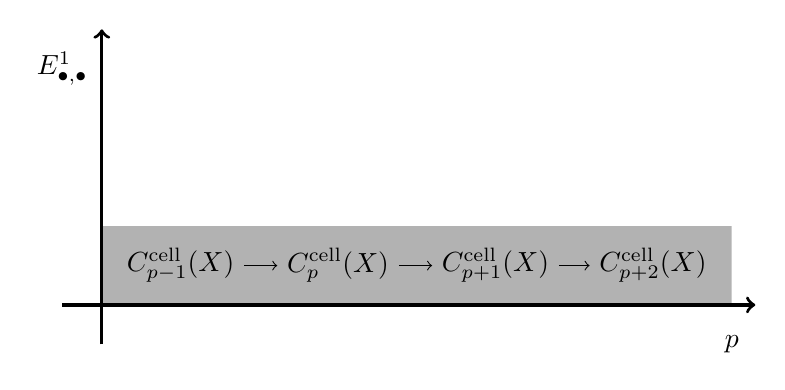
\begin{tikzpicture}
			\fill[opacity=0.3] (-1,-0.5) -- (-1,0.5) -- (7,0.5) -- (7,-0.5) -- (-1,-0.5);
			\draw[very thick, ->] (-1.5, -0.5) -- (7.3,-0.5);
			\draw[very thick, ->] (-1,-1) -- (-1,3);
			\draw 
%			(0,2) node(A){$E^{s,t}$} (2,2) node(C){$E^{s+1,t}$} (4,2) node{$\ast$} (6,2) node{$\ast$}
%			(0,1) node{$\ast$} (2,1) node{$\ast$} (4,1) node(D){$E^{s+2,t-1}$} (6,1) node{$\ast$}
			(0,0) node(A){$C_{p-1}^{\mathrm{cell}}(X)$} (2,0) node(B){$C_{p}^{\mathrm{cell}}(X)$} (4,0) node(C){$C_{p+1}^{\mathrm{cell}}(X)$} (6,0) node(D){$C_{p+2}^{\mathrm{cell}}(X)$};
			\draw 
			(-1.5,2.5) node{$E^{1}_{\bullet,\bullet}$} (7,-1) node{$p$};
			
			\draw[->] (A) --node[anchor=south]{$\de$} (B);
			\draw[->] (B) --node[anchor=south]{$\de$} (C);
			\draw[->] (C) --node[anchor=south]{$\de$} (D);
		\end{tikzpicture}
		\caption{La prima pagina della successione 
		spettrale nella \hyperref[h-cell]{Proposizione~\ref{h-cell}}.}
    	\label{cell-e1}
	\end{figure}
	\end{proof}
\end{prop}

\begin{ex!}[\textbf{Bicomplessi}]
	Alcuni oggetti che permettono di generare successioni spettrali come
	spiegato nel \hyperref[SS-machine]{Teorema~\ref{SS-machine}}
	sono i \emph{bicomplessi}.
	\begin{df}
		Un \textbf{bicomplesso} $(M,d^{h},d^{v})$ (o \textbf{complesso doppio})
		è un $R$-modulo bigraduato $M_{\bullet,\bullet}$
		dotato di due differenziali
		\begin{equation*}
			d^{h}_{p,q}: M_{p,q} \longrightarrow M_{p-1,q}\,, \quad
			d^{v}_{p,q}: M_{p,q} \longrightarrow M_{p,q-1}\,,
		\end{equation*}
		di bigrado $(0,-1)$ e $(-1,0)$ rispettivamente\footnote{Quello definito è un bicomplesso con notazione omologica; è facile adattare la definizione al caso coomologico considerando differenziali di bigrado $(0,1)$ e $(1,0)$ rispettivamente.},
		tali che $d^{h}d^{v} + d^{v}d^{h}=0$, ovvero ogni quadrato della griglia
		è \emph{anticommutativo}.
		\begin{equation*}
			\begin{tikzcd}
      & \dots \arrow[d]                        & \dots \arrow[d]                              &                 \\
\dots & {M_{p-1,q}} \arrow[d, "d^v"] \arrow[l] & {M_{p,q}} \arrow[d, "d^v"] \arrow[l, "d^h"'] & \dots \arrow[l] \\
\dots & {M_{p-1,q-1}} \arrow[d] \arrow[l]      & {M_{p,q-1}} \arrow[l, "d^h"] \arrow[d]       & \dots \arrow[l] \\
      & \dots                                  & \dots                                        &                
\end{tikzcd}
		\end{equation*}
		Dato un bicomplesso $M$, il suo \textbf{complesso totale} $\cat{tot}(M)$
	è l'$R$-modulo graduato dato da
	\begin{equation*}
		\cat{tot}(M)_{n} := \bigoplus_{p \in \Z} M_{s,n-s}\,,
	\end{equation*}
	dotato del \textbf{differenziale totale} $d = d^{v} + d^{h}$.
	\end{df}
	
	Quando ci viene dato un bicomplesso $M$, possiamo calcolare la sua omologia
	lungo due diverse direzioni: infatti, abbiamo l'omologia \emph{orizzontale}
	$H^{I}_{*,*}(M) := H(M_{\bullet, \bullet}, d^{h})$
	e l'omologia \emph{verticale} $H^{II}_{*,*}(M) := H(M_{\bullet, \bullet}, d^{v})$.
	La condizione $d^{h}d^{v} + d^{v}d^{h}=0$ che definisce il bicomplesso
	garantisce che il differenziale $d^{v}$ induce un differenziale verticale
	$\overline{d^{v}}$ su $H^{I}_{*,*}(M)$; analogamente, anche
	$H^{II}_{*,*}(M)$ ottiene un differenziale $\overline{d^{h}}$.
	Possiamo dunque calcolare nuovamente l'omologia di questi due complessi
	e ottenere così
	\begin{equation*}
		H^{II}_{*,*}H^{I}(M) := H\left(H^{I}_{*,*}(M), \overline{d^{v}}\right)\,, \quad
		H^{I}_{*,*}H^{II}(M) := H\left(H^{II}_{*,*}(M), \overline{d^{h}}\right)\,.
	\end{equation*}
	Questi due procedimenti danno due diverse successioni spettrali,
	le quali sono legate a $H_{*}(\cat{tot}(M))$ come spiegato nel seguente
	
	\begin{thm}\label{SS-bicomplex}
		Dato un bicomplesso $(M,d^{h},d^{v})$, esistono due successioni
		spettrali $\{ {}^{I}E^{r}_{\bullet,\bullet}, {}^{I}d^{r}\}$
		e $\{ {}^{II}E^{r}_{\bullet,\bullet}, {}^{II}d^{r}\}$, tali che
		\begin{equation*}
			 {}^{I}E^{2}_{\bullet,\bullet} \simeq H^{I}_{*,*}H^{II}(M) \,,
			 \quad  {}^{II}E^{2}_{\bullet,\bullet} \simeq H^{II}_{*,*}H^{I}(M)\,.
		\end{equation*}
		Se $M$ è concentrato nel primo quadrante, allora entrambe le successioni
		sopra convergono a $H_{*}(\cat{tot}(M))$.
		\begin{proof}
			È sufficiente dimostrare il Teorema per 
			$\{ {}^{I}E^{r}_{\bullet,\bullet}, {}^{I}d^{r}\}$,
			dato che l'altro caso è simmetrico. 
			L'idea è quella di sfruttare il \hyperref[SS-machine]{Teorema~\ref{SS-machine}}
			con $A = \cat{tot}(M)$ e $d$ il suo differenziale totale. 
			Definiamo quindi le filtrazioni sul complesso totale
			\begin{equation*}
				F^{I}_{p}\left( \cat{tot}(M) \right)_{q} := \bigoplus_{r \le p} M_{r,q-r}\,,
				\quad
				F^{II}_{p}\left( \cat{tot}(M) \right)_{q} := \bigoplus_{r \le p} M_{q-r,r}\,,
			\end{equation*}
			dove $F^{I}$ viene detta \textbf{filtrazione per colonne},
			mentre $F^{II}$ viene detta \textbf{filtrazione per righe}.
			
			\missingfigure{Add image of filtration}
			
			Per prima cosa identifichiamo la prima pagina della successione:
			notiamo che per ogni $p,q \in \Z$ la filtrazione dà il quoziente
			\begin{equation*}
					\left( \frac{F_{p}^{I}(\cat{tot}(M))}{F_{p-1}^{I}(\cat{tot}(M))} \right)_{p+q}
					=  \frac{\bigoplus_{r \le p} M_{r, p + q - r}}{\bigoplus_{r \le p-1} M_{r,p+q-r}}
					% \simeq \left( M_{p,\bullet} \right)_{p+q}
					\simeq M_{p,q}\,,
			\end{equation*}
			quindi la tripla $\big(F^{I}_{p}(\cat{tot}(M)), F^{I}_{p-1}(\cat{tot}(M)), 
			F^{I}_{p-2}(\cat{tot}(M))\big)$ dà la successione esatta di complessi
			\begin{equation*}
				\begin{tikzcd}
					\cat{0} \ar[r]
					& M_{p-1,\bullet} \ar[r]
					& M_{p-1,\bullet} \oplus M_{p,\bullet} \ar[r]
					& M_{p,\bullet} \ar[r]
					& \cat{0}\,,
				\end{tikzcd}
			\end{equation*}
			ognuno dei quali è dotato del \emph{differenziale verticale} $d^{v}$,
			quindi grazie al \textbf{Lemma del Serpente} si ottiene
			\begin{equation*}
				\begin{tikzcd}[column sep=small]
					\dots \ar[r]
					& H_{p+q}(M_{p,\bullet}, d^{v}) = H^{II}_{p,q}(M) \ar[r, "\delta"]
					& H_{p+q-1}(M_{p-1,\bullet}, d^{v}) = H^{II}_{p-1,q}(M) \ar[r]
					& \dots
				\end{tikzcd}
			\end{equation*}
			dove si verifica che $\delta = \overline{d^{h}}$. Si deduce quindi che
			${}^{I}E_{\bullet,\bullet}^{1} \simeq H^{II}_{*,*}(M)$, 
			da cui si conclude che
			\begin{equation*}
				{}^{I}E_{\bullet,\bullet}^{2} \simeq H^{I}_{*,*}H^{II}(M)\,.
			\end{equation*}
			
			Infine, se $M$ è concentrato nel primo quadrante, 
			la filtrazione $F^{I}$ è limitata sia dal basso, sia dall'alto,
			dato che per ogni $t \in \Z$ vale
			\begin{equation*}
				\cat{tot}(M)_{t} =  F^{I}_{t}\cat{tot}(M)_{t} 
				\supset F^{I}_{t-1}\cat{tot}(M)_{t}
				\supset \dots \supset F^{I}_{0}\cat{tot}(M)_{t} 
				= M_{0,t} \supset F^{I}_{-1}\cat{tot}(M)_{t}  = 0\,,
			\end{equation*}			
			quindi per il \hyperref[SS-machine]{Teorema~\ref{SS-machine}}
			la successione converge a $H(\cat{tot}(M))$.
%			\begin{equation*}
%				\frac{F_{p}H_{p+q}(\cat{tot}(M))}{F_{p-1}H_{p+q}(\cat{tot}(M))}
%				=  \frac{\bigoplus_{r \le p} M_{r, p + q - r}}{\bigoplus_{r \le p-1} M_{r,p+q-r}}
%					% \simeq \left( M_{p,\bullet} \right)_{p+q}
%					\simeq H_{p+q}(\cat{tot}(M))\,.
%			\end{equation*}
		\end{proof}
	\end{thm}
\end{ex!}

\begin{ex!}[\textbf{Formula di Künneth}]
	Dati $(C_{\bullet},d)$ e $(D_{\bullet},\de)$ due complessi di catene su un campo $\KK$,
	consideriamo il bicomplesso $C_{\bullet} \otimes D_{\bullet}$ avente i differenziali
	\begin{equation*}
		d^{h}(x \otimes y) := dx \otimes y\,, \quad 
		d^{v}(x \otimes y) := (-1)^{\lvert x \rvert} x \otimes \de y\,.
	\end{equation*}
	Il suo complesso totale $T_{\bullet} := 
	\cat{tot}\left( C_{\bullet} \otimes D_{\bullet} \right)$
	è quindi dotato del differenziale
%	allora per ogni $n \in \Z$ vale
%	\begin{equation}\label{kunneth}
%		H_{n}\left( C_{\bullet} \otimes D_{\bullet} \right)
%		= \left( H_{*}(C_{\bullet}) \otimes H_{*}(D_{\bullet}) \right)_{n}\,.
%	\end{equation}
%	\begin{proof}
%		Ricordiamo che $T_{\bullet} := C_{\bullet} \otimes D_{\bullet}$ è
%		il complesso di catene dato in grado $q$ da
%		\begin{equation*}
%			T_{q} = \bigoplus_{i+j=q}C_{i} \otimes_{\KK} D_{j}\,,
%		\end{equation*}
%		dotato del differenziale
		\begin{equation*}
			D(x \otimes y) := dx \otimes y + (-1)^{\lvert x \rvert} x \otimes \de y \,,
		\end{equation*}
		e se si considera la filtrazione per colonne su $T_{\bullet}$, 
		data da
		\begin{equation*}
			F_{p}^{I}(T_{q}) := \bigoplus_{r \le p} C_{i} \otimes_{\KK} D_{q-r}\,,
		\end{equation*}
		allora per il \hyperref[SS-bicomplex]{Teorema~\ref{SS-bicomplex}}
		sappiamo che la successione spettrale associata converge a $H_{*}(T_{\bullet})$.
		Studiamo dunque le prime pagine della successione:
		la $0$-esima pagina è definita da $E^{0}_{p,q} := C_{p} \otimes_{\KK} D_{q}$,
		con differenziale $d^{0} := (-1)^{p} \cat{1}_{C} \otimes \de$,
		quindi si ottiene $E^{1}_{p,q} = C_{p} \otimes_{\KK} H_{q}(D_{*})$.
		Segue dal \hyperref[SS-machine]{Teorema~\ref{SS-machine}} che
		il differenziale $d^{1} = d \otimes \cat{1}_{H_{*}(D)}$,
		quindi la seconda pagina sarà 
		$E^{2}_{p,q} = H_{p}(C_{\bullet}) \otimes H_{q}(D_{\bullet})$
		con differenziali tutti nulli.
		Dato che $E_{\bullet,\bullet}^{2} = E_{\bullet, \bullet}^{\infty}$, 
		allora si ottiene la \textbf{Formula di Künneth}
	\begin{equation}\label{kunneth}
		H_{n}\left( C_{\bullet} \otimes D_{\bullet} \right)
		= \bigoplus_{p+q=n} H_{p}(C_{\bullet}) \otimes_{\KK} H_{q}(D_{\bullet}) 
		= \big(  H_{*}(C_{\bullet}) \otimes H_{*}(D_{\bullet}) \big)_{n} \,.
	\end{equation}
%	\end{proof}
\end{ex!}

\begin{ex!}[\textbf{Complesso di \v{C}ech-de Rham}]
	Dimostriamo che esiste un isomorfismo tra la 
	\textbf{coomologia di \v{C}ech} e la \textbf{coomologia di de Rham}
	di una varietà differenziabile reale. 
	Ricordiamo prima alcune nozioni:
	
	\begin{df}
		Data $M$ una varietà differenziabile reale,
		denotiamo con $\Omega^{k}(M)$ lo spazio delle $k$-forme
		$C^{\infty}$ su $M$, cioè lo spazio delle sezioni $C^{\infty}$
		del fibrato $\bigwedge^{k} T^{*}M$.
	\end{df}
	
	Ricordiamo che un elemento
		$\alpha \in \Omega^{k}(M)$ su un aperto coordinato
		è della forma
		\begin{equation*}
			\alpha = \sum_{|I| = k} \alpha_{I}(x) dx_{I}\,,
		\end{equation*}
		con $I$ il $k$-multiindice che rappresenta $i_{1} \le i_{2} \le \dots \le i_{k}$
		e $dx_{I} = dx_{i_{1}} \wedge dx_{i_{2}} \wedge \dots \wedge dx_{i_{k}}$.
		Localmente definiamo il \textbf{differenziale esterno} 
		$d : \Omega^{k}(M) \to \Omega^{k+1}(M)$ con la formula
		\begin{equation*}
			d\alpha = \sum_{j=1}^{n}\sum_{|I|=k} \frac{\de \alpha_{I}}{\de x_{j}}(x) \, 
			dx_{j} \wedge dx_{I}
		\end{equation*}
		e otteniamo il \textbf{complesso di de Rham} $(\Omega^{\bullet}(M),d)$,
		la cui coomologia sarà indicata con $H^{*}_{\mathrm{dR}}(M)$.
	
	\begin{lemma**}[Poincarè]
		Ogni forma chiusa su un aperto contraibile $A \subset \R^{n}$ è esatta.
		In altri termini, se $A$ è contraibile allora vale
		\begin{equation*}
			H^{k}_{\mathrm{dR}}(A) \simeq
			\begin{cases}
				\R\,, \quad &\text{se } k=0\,;\\
				0\,, \quad &\text{se } k>0\,.
			\end{cases}
		\end{equation*}
	\end{lemma**}
		
		Sia $M$ una varietà differenziabile e $\Uu$ un ricoprimento di $M$.
		Per una $k$-upla $U_{i_{1}}, \dots, U_{i_{k}} \in \Uu$, 
		indichiamo con $U_{i_{1}, \dots, i_{k}} := U_{i_{1}} \cap \dots \cap U_{i_{k}}$.
		
	\begin{df}
		Il \textbf{complesso di \v{C}ech a coefficienti reali} per $(M,\Uu)$ 
		è dato dagli $\R$-spazi vettoriali
		\begin{equation*}
			\v{C}_{\Uu}^{k}(M) := \bigoplus_{i_{0} \le \dots \le i_{k}} \underline{\R}(U_{i_{0}, \dots, i_{k}})\,,
		\end{equation*}
		dove $\underline{\R}$ è il fascio delle funzioni reali localmente costanti,
		sui quali definiamo i differenziali
		\begin{equation*}
			\delta^{k}: \v{C}^{k}_{\Uu}(M) \to \v{C}^{k+1}_{\Uu}(M)\,, \quad
			(\delta^{k}\alpha)_{i_{0}, \dots, i_{k+1}} :=
			\sum_{j=0}^{k+1} (-1)^{j} \alpha_{i_{0} \dots \hat{i_{j}} \dots i_{k+1}}\,.
		\end{equation*}
		Definiamo la \textbf{coomologia di \v{C}ech} subordinata al ricoprimento $\Uu$
		come
		\begin{equation*}
			\check{H}^{*}(M, \Uu) := H^{*}\left( \v{C}^{\bullet}_{\Uu}(M), \delta \right) \,.
		\end{equation*}
	\end{df}		
	
	Chiamiamo $\Uu$ un \textbf{buon ricoprimento} di $M$ se ogni aperto $U_{i} \in \Uu$
	è contraibile e ogni intersezione finita di aperti di $\Uu$ è vuota oppure contraibile.
		
	\begin{thm}
		Sia $M$ una $n$-varietà reale $C^{\infty}$ e $\Uu$ un buon ricoprimento per $M$.
		Allora la coomologia di \v{C}ech su $\Uu$ coincide con quella di De Rham,
		cioè esiste un isomorfismo naturale
		\begin{equation*}
			\check{H}^{*}(M;\Uu) \simeq H^{*}_{\mathrm{dR}}(M)\,.
		\end{equation*} 
		\begin{proof}
			Definiamo il \emph{complesso doppio di \v{C}ech-de Rham} come
			\begin{equation*}
				C^{p,q} := \prod_{i_{0} \le i_{1} \le \dots \le i_{p}} \Omega^{q}(U_{i_{0} \dots i_{p}})\,;
			\end{equation*}
%			su cui consideriamo il differenziale $D := \delta + (-1)^{p}d$.
			la pagina $E_{0}^{\bullet, \bullet}$ appare così:
			\begin{equation*}
				\begin{tikzcd}[column sep=small]
					\dots & & & \\
					\prod_{i_{0}} \Omega^{2}(U_{i_{0}}) \ar[r] \ar[u]
					&  \dots & & \\
					\prod_{i_{0}} \Omega^{1}(U_{i_{0}}) \ar[r, "\delta"] \ar[u, "d"] 
					& \prod_{i_{0} \le i_{1}} \Omega^{1}(U_{i_{0} i_{1}})  \ar[u, "d"] \ar[r] & \dots  & \\
					\prod_{i_{0}} \Omega^{0}(U_{i_{0}}) \ar[r, "\delta"] \ar[u, "d"] 
					& \prod_{i_{0} \le i_{1}} \Omega^{0}(U_{i_{0} i_{1}})  \ar[u, "d"] \ar[r] & 
					\prod_{i_{0} \le i_{1} \le i_{2}} \Omega^{0}(U_{i_{0} i_{1} i_{2}})  
					\ar[u] \ar[r] & \dots
				\end{tikzcd}
			\end{equation*}
			Prendiamo dunque il complesso totale $T^{\bullet}$ associato al bicomplesso,
			cioè
			\begin{equation*}
				T^{n} := (\cat{tot} \, C)_{n} = \bigoplus_{p+q=n} C^{p,q}\,,
			\end{equation*}
			con differenziale $D = \delta + (-1)^{p}d$, sul quale consideriamo due
			diverse filtrazioni:
			\begin{itemize}
				\item la filtrazione per colonne 
				$F^{p}_{I}T^{n} := \bigoplus_{r \ge p} T^{r,n-r}$
				induce su $E_{0}^{p,q} = C^{p,q}$ il
				differenziale $d_{0} = (-1)^{p}d$, quindi per
				il \hyperref[SS-bicomplex]{Teorema~\ref{SS-bicomplex}}
				la prima pagina è data da
				\begin{equation*}
				E_{1}^{p,q} 
				= H_{II}^{p,q}(C) 
				= \prod_{i_{0} \le \dots \le i_{p}} H_{\mathrm{dR}}^{q}(U_{i_{0} \dots i_{p}})
				= \begin{cases}
					\R\,, \quad &\text{se } q = 0\,; \\
					0\,, \quad &\text{altrimenti},
				\end{cases}
				\end{equation*}
				dove l'ultima uguaglianza segue dall'ipotesi di $\Uu$ buon ricoprimento.
				Si noti in particolare che
				\begin{equation*}
					H^{0}_{\mathrm{dR}}(U_{i_{0} \dots i_{p}}) 
					= \R
					= \underline{\R}(U_{i_{0} \dots i_{p}})
				\end{equation*}
				è dotato del differenziale  $d_{1}=\delta$. Dato che la successione
				collassa alla seconda pagina, 
				il limite è $E_{\infty}^{p,q} = E_{2}^{p,q}$,
				quindi si conclude che
				\begin{equation*}
				 	H^{*}(T^{bullet}) = \check{H}^{*}(M;\Uu)\,.
				 \end{equation*}
				
				\item Dalla filtrazione per righe 
				$F_{II}^{p}C^{n}=\bigoplus_{r \ge p} C^{n-r,r}$
				si ottiene $E_{0}^{p,q} = C^{p,q}$ con il differenziale $d_{0}=\delta$.
				
				\begin{lemma}
					C'è un'omotopia di catene
					\begin{equation*}
						\kappa : \prod_{i_{0} \le \dots \le i_{p}} \Omega^{\bullet} (U_{i_{0} \dots i_{p}})
						\longrightarrow \prod_{i_{0} \le \dots \le i_{p-1}} \Omega^{\bullet} (U_{i_{0} \dots i_{p-1}})
					\end{equation*}
					tra l'identità e la mappa nulla in grado $p > 0$.
					\begin{proof}
						Data $\{\rho_{i}\}_{i}$ una partizione dell'unità
						sbordinata a $\Uu$, 
						è sufficiente porre
						\begin{equation*}
							(\kappa \omega)_{i_{0} \dots i_{p-1}} 
							:= \sum_{i} \rho_{i} \, \omega_{i\,i_{0} \dots i_{p-1}}\,.
						\end{equation*}
						Infatti si verifica che per ogni $p > 0$ si ha
						\begin{align*}
							(\delta \kappa \omega)_{i_{0} \dots i_{p}}
							=& \sum_{j = 0}^{p} \sum_{i} (-1)^{j} \rho_{i} \, \omega_{i\,i_{0} \dots \hat{i_{j}} \dots i_{p}}\,, \\
							(\kappa \delta \omega)_{i_{0} \dots i_{p}}
							= \omega_{i_{0} \dots i_{p}} +& \sum_{i} \sum_{j = 0}^{p} (-1)^{j+1} \rho_{i} \, \omega_{i\,i_{0} \dots \hat{i_{j}} \dots i_{p}}\,,
						\end{align*}
						quindi $\delta \kappa + \kappa \delta = \cat{1}$.
					\end{proof}
				\end{lemma}
				
				Come conseguenza di questo \textbf{Lemma}, 
				segue che in $E^{p,q}_{1}$
				sopravvive solo la colonna $p=0$.
				Dato che $\ker \delta$ è costituito dalle $k$-forme \emph{globali},
				allora 
				\begin{equation*}
				E_{1}^{p,q} 
				= \begin{cases}
					\Omega^{q}(M) \,, \quad &\text{se } p = 0\,; \\
					0\,, \quad &\text{altrimenti},
				\end{cases}
				\end{equation*}
				e si verifica che il differenziale verticale è $d_{1}=d$ qdi de Rham.
				La successione collassa alla seconda pagina, per cui si ha
				\begin{equation*}
					E_{\infty}^{p,q} = E_{2}^{p,q}
					= \begin{cases}
						H_{\mathrm{dR}}^{q}(M)\,, \quad \text{se } p=0\,; \\
						0\,, \quad \text{altrimenti},
					\end{cases}
				\end{equation*}
				quindi concludiamo che $H^{*}(T^{\bullet}) = H_{\mathrm{dR}}^{*}(M)$.
			\end{itemize}
			Ricapitolando, abbiamo dimostrato che 
			$\check{H}^{*}(M;\Uu) = H^{*}(T^{\bullet}) = H_{\mathrm{dR}}^{*}(M)$.
		\end{proof}
	\end{thm}
\end{ex!}




